% !TEX TS-program = pdflatex
% !TEX encoding = UTF-8 Unicode

% This is a simple template for a LaTeX document using the "article" class.
% See "book", "report", "letter" for other types of document.

\documentclass[11pt]{article} % use larger type; default would be 10pt

\usepackage[utf8]{inputenc} % set input encoding (not needed with XeLaTeX)

%%% Examples of Article customizations
% These packages are optional, depending whether you want the features they provide.
% See the LaTeX Companion or other references for full information.

%%% PAGE DIMENSIONS
\usepackage{geometry} % to change the page dimensions
\geometry{a4paper} % or letterpaper (US) or a5paper or....
% \geometry{margin=2in} % for example, change the margins to 2 inches all round
% \geometry{landscape} % set up the page for landscape
%   read geometry.pdf for detailed page layout information

\usepackage{graphicx} % support the \includegraphics command and options
\usepackage{enumerate}


% \usepackage[parfill]{parskip} % Activate to begin paragraphs with an empty line rather than an indent

%%% PACKAGES
\usepackage{booktabs} % for much better looking tables
\usepackage{array} % for better arrays (eg matrices) in maths
\usepackage{paralist} % very flexible & customisable lists (eg. enumerate/itemize, etc.)
\usepackage{verbatim} % adds environment for commenting out blocks of text & for better verbatim
\usepackage{subfig} % make it possible to include more than one captioned figure/table in a single float
% These packages are all incorporated in the memoir class to one degree or another...

%%% HEADERS & FOOTERS
\usepackage{fancyhdr} % This should be set AFTER setting up the page geometry
\pagestyle{fancy} % options: empty , plain , fancy
\renewcommand{\headrulewidth}{0pt} % customise the layout...
\lhead{}\chead{}\rhead{}
\lfoot{}\cfoot{\thepage}\rfoot{}

%%% SECTION TITLE APPEARANCE
\usepackage{sectsty}
\allsectionsfont{\sffamily\mdseries\upshape} % (See the fntguide.pdf for font help)
% (This matches ConTeXt defaults)

%%% ToC (table of contents) APPEARANCE
\usepackage[nottoc,notlof,notlot]{tocbibind} % Put the bibliography in the ToC
\usepackage[titles,subfigure]{tocloft} % Alter the style of the Table of Contents
\renewcommand{\cftsecfont}{\rmfamily\mdseries\upshape}
\renewcommand{\cftsecpagefont}{\rmfamily\mdseries\upshape} % No bold!

%%% END Article customizations

%%% The "real" document content comes below...

\title{PoM Week 12\\Genaflevering}
\author{Martin Simon Haugaard\\cdl966}
%\date{} % Activate to display a given date or no date (if empty),
         % otherwise the current date is printed 

\begin{document}
\maketitle

\section*{12g}
\subsection{Bølgeligningen}
\subsubsection*{a}
Givet formlen:\\
$c^2 \frac{\vartheta^2}{\vartheta x^2}u(t,x) = \frac{\vartheta^2}{\vartheta t^2}u(x,t)$\\
\\
og approksimationerne\\
\\
$\frac{\vartheta^2}{\vartheta x^2} \approx \frac{u(x_{i+1}, t_j) - 2u(x_i, t_j) + u(x_{i-1}, t_j)}{h^2} $
\\
$\frac{\vartheta^2}{\vartheta t^2} \approx \frac{u(x_i, t_{j+1}) - 2u(x_i, t_j) + u(x_i, t_{j-1})}{k^2} $\\
\\
Det er muligt at se at der 5 forskellige led at operere med:
\begin{description}
\item[$U_1$:]{$u(x_{i+1}, t_j)$}
\item[$U_2$:]{$u(x_i, t_j)$}
\item[$U_3$:]{$u(x_{i-1}, t_j)$}
\item[$U_4$:]{$u(x_i, t_{j+1})$}
\item[$U_5$:]{$u(x_i, t_{j-1})$}
\end{description}
Og herudfra ser formlen således ud:\\
\\
$c^2\frac{U_1 - 2 U_2 + U_3}{h^2}=\frac{u_4 - 2 U_2 + U_5}{k^2}$\\
\\
Hvor vi ønsker at isolere $U_4$, hvilket giver følgende formel:\\
\\
$U_4 = \frac{c^2 k^2}{h^2}(U_1 - 2 U_2 + U_3) + 2 U_2 - U_5$\\
\\
Nu har vi så en formel til beregning af funktionen $u$ som funktion af $x$ til næste tidspunkt $t_{j+1}$.

\subsubsection*{c}
Her er så resultatet af min kørsel af programmet.\\ Følgende eksempler er ved \textit{h} samt \textit{k} på $0.5$\\
\begin{figure}[h!]
\centering
   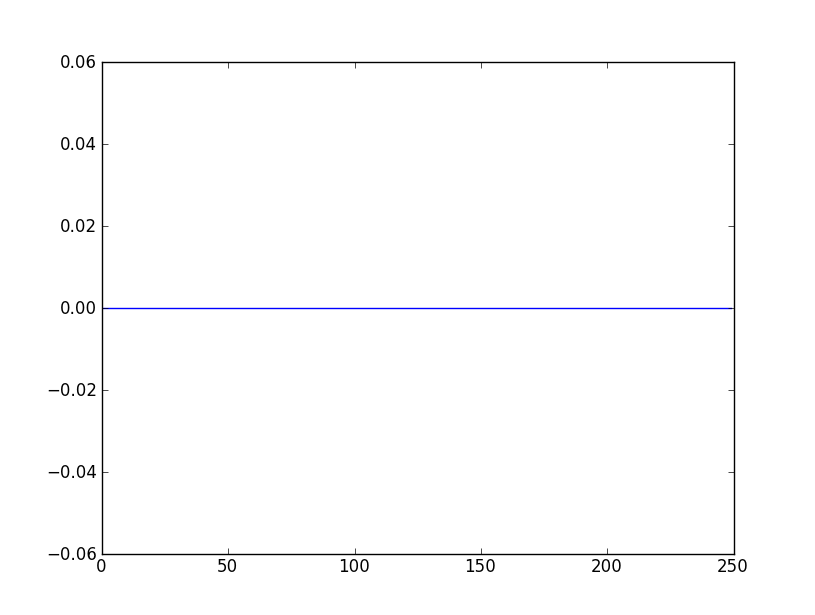
\includegraphics[width=0.5\textwidth]{bild1}
  \caption{Mit stadium uden nogen bølge i gang}
\end{figure}
\\Ovenfor ses et stadium, inden en bølge sættes i gang.
\\
\begin{figure}[h!]
\centering
   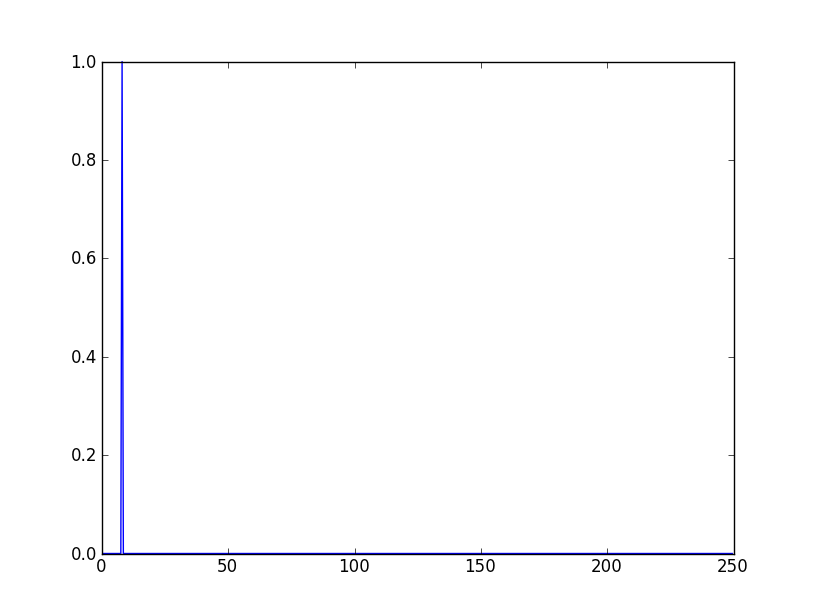
\includegraphics[width=0.5\textwidth]{bild2}
  \caption{Bølgen er startet!}
\end{figure}\\
Det er her tydeligt at se hvor bølgen befinder sig, da der kun er et udslag på grafen, netop der hvor bølgen befinder sig.
\newpage
Bevæger vi os et par iterationer frem ser bølgen således ud:
\begin{figure}[h!]
\centering
   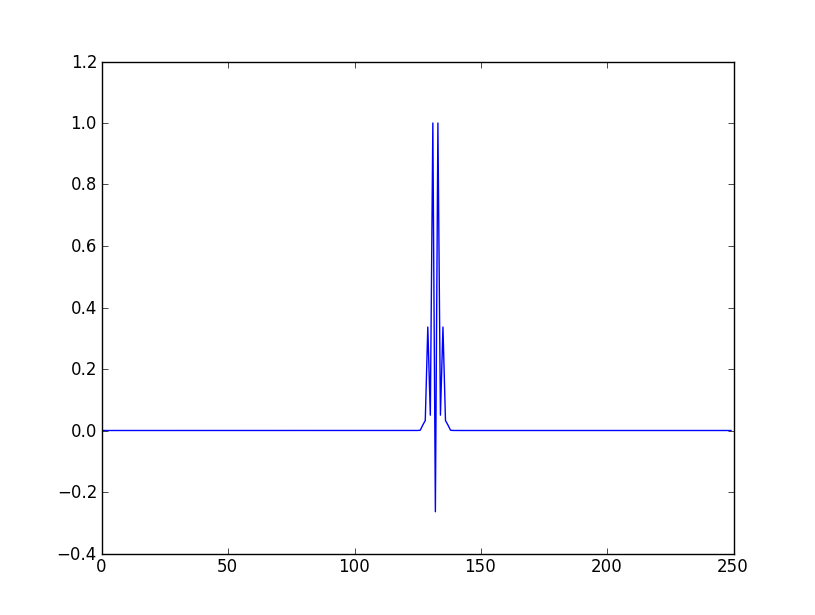
\includegraphics[width=0.5\textwidth]{midvejs}
  \caption{Vi er her 233 iterationer inde, og det ligner vi er halvvejs.\\
  Bemærk at der ikke blot er 250 sæder på stadium, da \textit{h} er sat til 0.5, er der to sæder pr værdi ved x-aksen.}
\end{figure}
\\
Bølgen er godt halvvejs, og sådan bliver den ellers ved med at bevæge sig rundt. Når den når til kanten, fortsætter den ved x-værdi 0 og starter sådan set forfra.
\\
\begin{figure}[h!]
\centering
   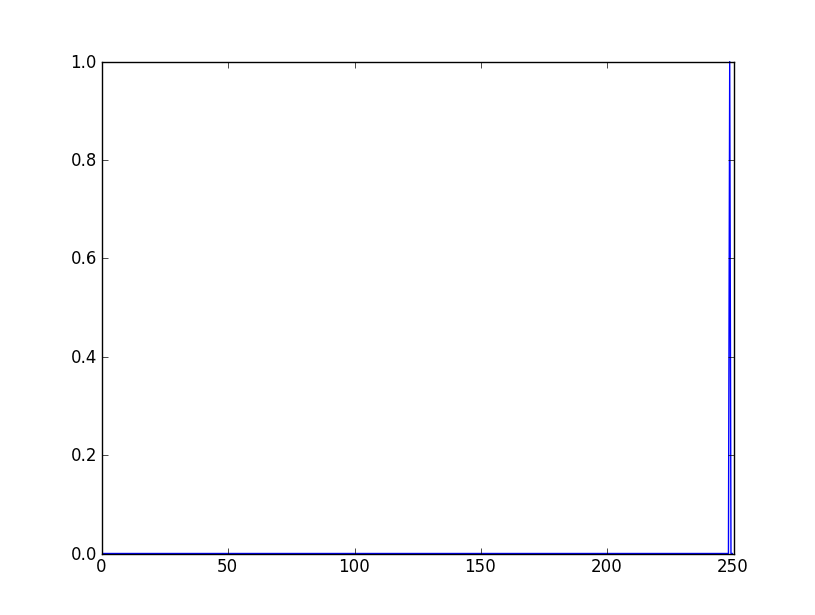
\includegraphics[width=0.5\textwidth]{slut}
  \caption{Bølgen har nået kanten af stadium, og vil begynde at wrappe rundt til starten.}
\end{figure}

\subsection*{Hvor land tid tager det for bølgen af nå kanten af stadium?}
Dette kommer an på hvor vores super-fan vælger at rejse sig. Hvis \textit{h} \& \textit{k} begge er initialiseret til 0.5
vil vores super-fan initialiseres på placering 16 på stadium, og bølgen har i alt 500 sæder den skal igennem.\\
Hvilket i alt tager 484 iterationer, hver af længden 0.5 tidsenhed. Altså tog det i alt \begin{math}484*0.5=\end{math} 242 tidsenheder, at bevæger bølgen igennem
hele stadium.

Skifter vi nu \textit{h} \& \textit{k} sat til 1.0, er vores super fan på sæde 8, og det tager 242 iterationer, af tidsenhed 1, at nå til kanten.
Altså tager et stadions længde, minus fan's startposition, at nå til enden af stadium, såfremd \textit{k} og \textit{k} er ens, og i begge disse eksempler var det altså 242 tidsenheder.

\subsection*{Hvad der der hvis \textit{h} eller \textit{k} ændres?}
Hvis \textit{h} formindskes, tilføjes der flere sæder til stadium. Altså er der flere mennesker der skal rejse sig før at bølgen når rundt, og modsat kommer der færre sæder hvis \textit{h} stiger\\
Hvis \textit{k} ændres til at være mindre, vil tidsintervallet imellem to iterationer blive mindre, altså vil bølgen tiltage i fart, da folk er blevet hurtigere til at rejse sig. Derimod hvis \textit{k} stiger, vil bølgen bevæge sig langosmmere.
\end{document}
